%!TEX program = pdflatex
% Full chain: pdflatex -> biber/bibtex -> pdflatex -> pdflatex
\documentclass[11pt,en]{elegantpaper}

\title{TEST}
\author{Yushuo Chen MAM, Jan 2024}

\usepackage{array}
\newcommand{\ccr}[1]{\makecell{{\color{#1}\rule{1cm}{1cm}}}}

\addbibresource[location=local]{reference.bib} % reference file
\begin{document}

\maketitle

\begin{abstract}
abstract
  \keywords{keywords}
\end{abstract}

\section{Introduction}
This challenge is based on the question B of \textit{2022 Mathematical Contest in Modeling}.
I will focus on part (3) of question 1.
And I will use ant-cycle algorithms to address the challenge rather than nonlinearly constrained optimization of very first attempt in 2022.

\section{Question Description}
The whole question is about positioning a group of unmanned aerial vehicle (UAV) during flying.
During the formation flight of UAVs formation, in order to avoid external interference, 
electromagnetic silence should be maintained as much as possible, reduce the emission of electromagnetic wave signals outward.
In UAVs formation, there are transmition group and acceptance group.
The transmition group is made of few UAVs to transmit signal and the rest of UAVs in acceptance group receive.
The signals must be the direction information from any other two sinal transmitting UAVs.
Each UAV in the formation has a fixed number, and its relative position with other UAVs remains unchanged in the formation.
E.g. In figure(a) the angle information of $\alpha_1,\;\alpha_2,\;\alpha_3$.
FY01, FY02, FY03 are in the transmition group and FY04 receives the angle informations.

\begin{figure}[htbp]
  \centering
  \subfigure[Direction information received]{
    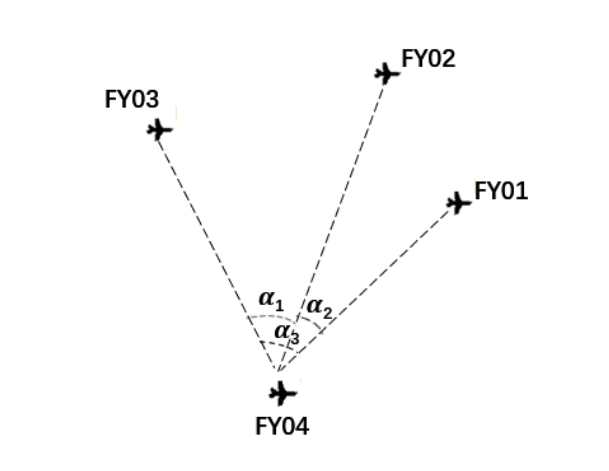
\includegraphics[scale=0.2]{direction information.png}
  }
  \subfigure[Circular UAVs formation]{
    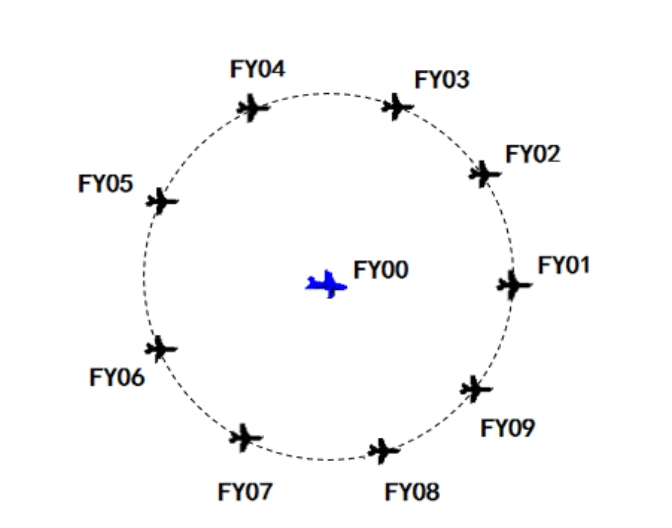
\includegraphics[scale=0.2]{circular formation.png}
  }
\end{figure}

The flying formation is made of 10 UAVs and forms a circular formation.
They are all flying at the same height level. 
In this circular formation, 9 UAVs locat on the circle, and one UAV (\textit{No.FY00}) is on the center. Like ligure(b).
\par
The initial situation is that all UAVs except FY00 arenot at the right positions.
\footnote{The initial positions can be found in \url{https://github.com/CyanCap/CI-code.git}}
Now, in order to adjust the positions, we are limited to choosing FY00 and 2 UAVs on the circle to transmit signals.
After times of adjustments, make 9 UAVs uniformly distributed on the circle. 
We need to give a specific plan.

\section{Symbol Description}
\begin{center}
  \setlength{\tabcolsep}{9mm}{
    \begin{tabular}{ccc}
      \toprule  %headline
      \textbf{Symbol} & \textbf{Discription}\\
      \midrule  %line
      FY00  & origin UAV\\
      FY0i  & i-th UAVs around FY00\\
      $\alpha_{1,\; 2,\; 3}$  & angle informations / rad\\
      $L_i$ & polar coordinate of i-th UAV / $(m,\; ^{\circ})$\\
      \bottomrule %buttumline
  \end{tabular}}
\end{center}

\section{Combination of Swarm Intelligence And Evolutionary Computing}
In 2022 modeling contest, we solve the location model before solving this problem.
So we only need to consider how to adjust positions only with signal informations based on ant-cycle algorithm.
\subsection{Question Analysis}
In this question, we first need to choose the transmition UAVs to send signals.
FY00 and FY01 can be chosen since they are in the correct positions.
we should assume that the selected UAVs are in the correct position by default, although error must exist.
When signals acceptance happens, based on the locations, we can consider it as an optimization problem.
Set up a polar coordinate system with UAV FY00 as origin.
So the coordinate of it is $(0,0)$ in $(m,^{\circ})$
The objective function can be considered as 
\[
  min\;\; f_i^T = -\frac{\sqrt{ h_i^2 + \Delta r_i^2}}{T},
  \]
where $\Delta r_i$ means the error radius of FY0i between adjusted position and correct position, and $T$ means iteration times.
And 
\begin{align*}
  h_i = R\lvert \Delta \theta_i \rvert
\end{align*}
Remark: $h_i^2$ and $\Delta r_i^2$ are quadratic form of variables i.e. $h_i^2 = h_i\cdot h_i$.\\
We want to minimize the error to ensure the accuracy, with the consideration of transmition times.
This is because the more transmition is made, the higher possibility of disturb due to unnecessary noise.

\subsection{Choice of Method}
I am more likely to use GREEDY algorithm to choose which UAVs to transmit signals.
Rather than address it as nonlinearly constrained optimization which was stated in my contest thesis,
I would like to tackle it using swarm intelligence studied in lecture.
9 UAVs around FY00 can be considered as a population operating in the same optimization direction.
And this optimal goal is that 9 UAVs are in the positions uniformly locating on the cycle.
Moreover, inherited informations from the previous generation take a great importance in genetic algorithms (GA).
And since errors in this formation are on a small order of magnitude, using GA will not require a huge searching space 
if we generate it in a relatively big measure unit.

\section{Process And Encoding}
In this question, let's encoding adjustments first.
After the transmition part, we can obtain the whole locations of 10 UAVs in the polar system.
E.g. \[L_0^0=(0,0),\; L_1^0=(100,0),\; L_2^0=(98,40.10)\] where $L_i^j$ means the position of $i$-th UAV in iteration $j$.
\\ \textbf{Especially}, every time the UAVs transmit signals we assume these UAVs are in the correct positions.
For example, in initial situation we choose FY00, FY01, FY02 to transmit signals.
Then FY02 is considered in the correct position which is $L_2^0 = (100,40)$.
Due to this, 10 UAVs' positions are not exactly the true positions, but a approximate value.
\\Think of 9 UAVs are 9 ants. So they are all placed well.
A adjustment determine an ant path, then leave pheromone along the path.
Then compare the new adjustment direction and previous path with updating pheromone evaporation.
While different ants will be computed to fitness using objective function $f_i =-\frac{\sqrt{ h_i^2 + \Delta r_i^2}}{T} $.
This will guild us to select well performed parents and do genetic operators.
\\Now turn to the easier part about choosing the transmition UAVs.
Everytime we pick UAVs with minimal objective function i.e. fitness to be in the transmition group.

\section{Ant-cycle Algorithm}
\subsection{Previous Work}
The location model need to be generated by using $\alpha_1,\; \alpha_2,\; \alpha_3$ and 3 transmition UAVs' coordinates
$(100,\; \theta_i)$.
Remember, we assume transmitional UAVs are in the correct positions.
Since the focus is to adjust the positions, so I will state the location model as following.
\begin{align}
\left\{ 
    \begin{aligned}
    &\theta_k = \arctan \frac{\sin\alpha_3 \sin(\alpha_1 + \theta_i)-\sin\alpha_1 \sin(\alpha_3 -\theta_j)}{\sin\alpha_1 \sin(\alpha_3 - \theta_j)+\sin\alpha_3 \sin(\alpha_1 +\theta_i)}\\
    &r_k = \frac{R\sin(\alpha_1+(\theta_k - \theta_i))}{\sin\alpha_1}\\
    &\lvert \theta_k -\frac{2}{9}\pi \cdot(k-1) \rvert <\frac{50}{180}rad,\; \lvert r_k -R \rvert < 14\\
    &R=100.\; i,\; j,\; k\in[1,9],\;i\neq j\neq k
    \end{aligned} 
\right.
\end{align} 

where $r_k$ and $\theta_k$ are coordinates for k-th UAV. 
Though this location model, we can get any drone's location by using 3 UAVs to transmit signals.
We will apply these equation system directly in the rest of report.

\subsection{Modeling for Ant-cycle AS}
AS is developed by ACO (ant colony optimization).
It simulates the swarm of ants finding foods according the pheromones they leave.
Each ant's decision is based on a probability\\
Using the above location model, we can obtain all coordinates which are represented as $(r_i,\; \theta_i)_T$.
$T$ means the iteration.
With the actual coordinates data, objective functions for all UAVs could be calculated.
Fitness is generated by 
\[
  f_i^T =-\frac{\sqrt{ h_i^2 + \Delta r_i^2}}{T}.
\]
Then fitness will determine the direction to adjust.
At the first iteration, since there is no genetic information from the last iteration, so we can just do the adjustments though coordinates.
We record the direction which can be represented as polar vector $(\hat{r}_i,\; \hat{\theta}_i)_T$.\\
\textit{\textbf{Extra note}: polar vector could be added up and do the scaler multiplication i.e. $\lambda \cdot (\hat{r}_i,\; \hat{\theta}_i)$\\}
Using this and pheromone indicator $\tau$, we can get new direction linear combined with previous directions of UAV i.
\begin{align*}
  (\hat{r}_i,\; \hat{\theta}_i)_T = \sum_0^{T-1} \tau(t)\cdot (\hat{r}_i,\; \hat{\theta}_i)_t
\end{align*}
Also in AS, $\tau$ will be genreated by the pheromone updation.
So we have 
\begin{align*}
  \tau_i(t+1) = (1-\rho)\cdot \tau_i(t) +\sum_{0}^{T-1}\Delta \tau_i^k(t)
\end{align*}
where
\begin{align*}
  \Delta \tau_i^T = \frac{Q}{f_i^T}
\end{align*}
$\tau_i(T)$ means amount of pheromones of i-th drone at the iteration T.
$Q$ is the power of pheromones and $f_i^T$ is fitness of i-th UAV at iteration T.
Secondly, since we not only need to consider the correct direction of each choice, 
but also need to think of the minimal distance and the informationan ant walks so far.

After new directions are constructed by genetic algorithm, each ant will be able to choose one of them to go to.
This introduce the probability function:
\begin{align}
  p_i^k (t) =\frac{\tau_i^{\alpha}(t) \eta_i^{\beta}(t)}{\sum_0^T \tau_i^\alpha (t) \eta_i^{\beta}(t)}
\end{align} 
where $\eta_i(t)$ is the factor that represents heuristic information.
Then we should choose the way updating the pheromone as iteration $T$ goes by.

\subsection{Consistency of Direction}
Not like the other algorithm or classical SI, this question is a ``time series'' question.
Every actions done in the previous will affect the next iterations.
At the same time, 10 UAVs or 10 individuals must step in same pace to make sure this ``popluation'' optimize towards
the final solution.
In other words, one successful population share knowledge inside and build up correct evolutionary direction.
To reflect in this question, adjustment should consider the movement which other UAVs generate.
So we need to add up an accumulated parameter to make model perform better.
Which can be clarified as 
\begin{align*}
  (\hat{r}_i,\; \hat{\theta}_i)_T = \sum_{i=1}^{9} \sum_{j=1}^{T-1} \tau_j(t)\cdot (\hat{r}_j,\; (\lvert j-i\rvert)40^{\circ}\cdot\hat{\theta}_j)_T
\end{align*}
It means for every UAV, we consider the adjustment directions other UAVs make.
Then I think all requirements are well prepared. We can begin our algorithm to address the problem.

\subsection{Algorithm Design With Pseudo Code And Parameters}
Here is my pseudo code:
\par
\begin{algorithm}[H]
    \caption{Ant-cycle Ant System}
    \KwIn{$\alpha$, $\beta$, $\rho$, $Q$, $\tau_0$, $\eta$}
    \KwData{10 UAVs positions in the forms of $(r_i,\; \theta_i)$}
    \KwResult{iteration $T$, each adjustment $adj_T$ for iterations}
    Initialization\;
    \While{stopping condition is false}{
        GREEDY to choose UAVs transmit signals\;
        Evaluation function - fitness\;
        Genetic operators - combination of adjustment directions\;
        DO adjustments\;
        Evaporate and update pheromone\;
        Record the adjustments\;
        }
\end{algorithm}
\par
Now we should set all parameters which must fit our algorithm and problem better.
\begin{itemize}
  \item First initializtion using regularization and do tricky technique to make it positive.
  This can make the general application to make sense.
  \item Decision process biases: $\alpha = 4$, $\beta = 0.5$.
  Since the adjustments must be more accurate and efficient, $\tau^{\alpha}$ is more important.
  \item Factor of pheromone evaporate: $\rho = 0.8$.
  Pheromones should last short time because that we want the current calculation to be reserve after setting $\alpha$ and $\beta$.
  \item Factor indicating power of pheromone: $Q = 50$.
  \item Stopping condition is: total error is small than 2\%.
\end{itemize}

\section{Approach and More Discussions}
\subsection{Final Result}

\begin{figure}[htbp]
  \centering
  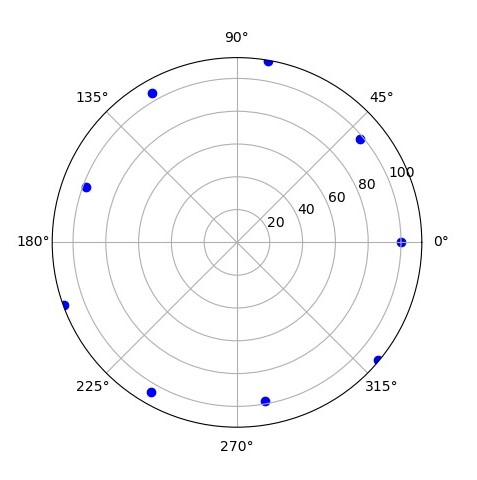
\includegraphics[scale=0.35]{initial location.jpg}
  \caption{initial location}
\end{figure}

Generating the algorithm with MATLAB, we could plot the final sketch map.

\begin{figure}[htbp]
  \centering
  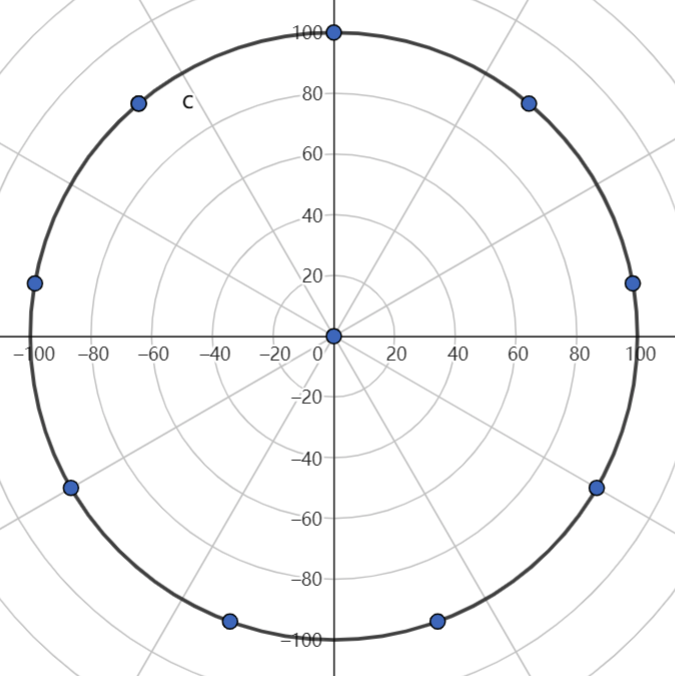
\includegraphics[scale=0.36]{final location.jpg}
  \caption{final location}
\end{figure}

And we have generate 5 times to get the final result.
And the total movement is 
\begin{center}
	\begin{tabular}{|c|c|c|}
		\hline
		\mbox{UAV No.}&\mbox{adjustment of $\theta_i$ / rad}&\mbox{adjustment distance / m}\\
		\hline
		FY01&2.81247324225734e-07&0\\
		\hline
		FY02&-0.0999997187526758&2.00744921022749\\
		\hline
		FY03&-0.209999718752676&12.0062673660278\\
		\hline
		FY04&0.250000281247324&5.01995072827991\\
		\hline
		FY05&0.140000281247324&2.01457467470591\\
		\hline
		FY06&0.0400002812473243&12.0002274487071\\
		\hline
		FY07&-0.0699997187526758&5.00156699828755\\
		\hline
		FY08&-0.169999718752676&2.02145328832454\\
		\hline
		FY09&-0.279999718752676&12.0111397208718\\
		\hline
	\end{tabular}
\end{center}

\subsection{Evaluation}
After we get the result, an good evaluation is necessary.
I choose the total error to be the estimator.
Apply as followed
\begin{align*}
  \sum_{i=1}^{9} (\bar{r_i} - r_i)^2 + (\bar{\theta_i}-\theta_i)^2.
\end{align*}
So the final error is $0.0007$.
It is a very small error and this model has performed well in this problem.
We could claim that all UAVs almost in the correct positions.\\
Besides, we add up all movement and get the total adjustment is $d=52.08263$ metres.
And this may indicate the difficulty of adjustment.
Less distance will be prefered.

\subsection{More Discussions}
When finishing this approach using SI, I rarely feel that this method may be not the best way to process.
In tranditional way, solve equations system to get a more accurate approximate solution.

Firstly, the topological relationship is not so clear since there is no given line or exact point location.
Ant Algorithm seems to search in an uncountable infinite set with a very small size of individuals (UAVs).
This is not encouraged in mathematics.
Secondly, although intelligence algorithms are also give a approximate solution, they are likely
to handle ``unexplored area'' or optimal solution without exact destination.
For example, when applying SI or EC to TSP we do not know the solution, and we need ants to find it.
But the destinations of UAVs are known, e.g. FY02 goes to $(100,\;40)$.
After a glance at the solutions on the internet, they indeed perform better than my estimation.

\printbibliography[heading=bibintoc, title=\ebibname]

% \appendix
% \appendixpage
% \addappheadtotoc


\end{document}
